\chapter[Resultados Gerais]{Resultados Gerais (Todas Empresas)}

\section{Considerações Iniciais}
Seguindo os passos apresentados no capítulo anterior, nós iremos mostrar os resultados da aplicação da pesquisa, a seleção de características executada no conjunto de dados gerados por essa pesquisa e a aplicação dos classificadores e suas respectivas acurácias na classificação dos desenvolvedores.

\section{Pesquisa}\label{secao4.2}
Primeiramente nós iremos apresentar os dados coletados com a pesquisa. Onze respondentes (supervisores) forneceram 61 respostas (avaliações únicas de desenvolvedores). Em alguns casos, alguns supervisores trabalham na mesma empresa, porém eles supervisionam diferente times. No total, oito empresas foram envolvidas na coleta de dados.

Nós pedimos para os supervisores classificarem os desenvolvedores em 5 graus de importância. Esses graus de importância e a distribuição dos desenvolvedores avaliados neles é mostrado na \autoref{fig_3}.

\begin{figure}[p]
	\centering
	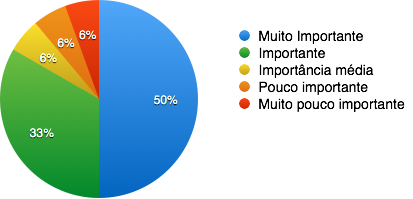
\includegraphics[width=\textwidth]{figs/geral/imagem-classe-original.png}
	\caption{\label{fig_3}Distribuição dos desenvolvedores avaliados pelas classes de importância}
\end{figure}

Analisando os resultados da pesquisa, nós chegamos à conclusão que os supervisores foram, em certo nível, conservadores em classificar seus desenvolvedores nas classificações mais baixas de importância.

A partir dessa análise, juntamente com a análise da matriz de confusão gerada pela aplicação dos algoritmos descritos na seção \ref{secao3.4} , nós decidimos agrupar os desenvolvedores em apenas duas classes, baseadas nas cinco classes originais de importância, como mostrado na \autoref{tabela3}, com o intuito de obter uma análise mais realística.

%inserir tabela 3

\begin{table}[h]
	\caption{Novo conjunto de classes de desenvolvedores}
	\label{tabela3}
	\def\arraystretch{1.5}
	\begin{tabular}{|p{6cm}|p{8.5cm}|}
		\hline
		\textbf{Novo conjunto de classes}  & \textbf{Conjunto de classes originais} \\ \hline
		\multirow{2}{*}{Alta importância}  & Muito importante                       \\ \cline{2-2} 
		& Importante                             \\ \hline
		\multirow{3}{*}{Baixa importância} & Importância média                      \\ \cline{2-2} 
		& Pouco importante                       \\ \cline{2-2} 
		& Muito pouco importante                 \\ \hline
	\end{tabular}
\end{table}

Utilizando esse novo conjunto de classes para agrupar os desenvolvedores, obtivemos a distribuição mostrada na \autoref{fig_4}.

\begin{figure}[p]
	\centering
	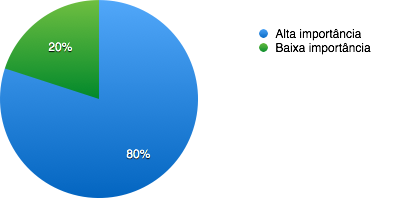
\includegraphics[width=\textwidth]{figs/geral/imagem-classe-alternativa.png}
	\caption{\label{fig_4}Distribuição dos desenvolvedores avaliados pela nova classe de importância}
\end{figure}

\section{Seleção de Características}\label{secao4.3}

Como explicado na seção \ref{secao3.3} , nós usamos o algoritmo GainRatio para ordenar os atributos propostos, para prosseguirmos com a seleção de características. A \autoref{tabela4} mostra as características ordenadas pelo mérito médio (um grau de influência do atributo na classificação, calculado pelo algoritmo) resultante da aplicação do algoritmo usando as classes originais e a \autoref{tabela5} mostra a mesma visão, utilizando agora as novas classes.

%inserir Tabela 4
\begin{table}[h]
	\caption{Ordenação dos atributos (conjunto original de 5 classes)}
	\label{tabela4}
	\def\arraystretch{2}
	\begin{tabular}{|p{8.5cm}|>{\centering\arraybackslash}p{3cm}|>{\centering\arraybackslash}p{3cm}|}
		\hline
		\textbf{Atributos}                                                      & \textbf{Posição média} & \textbf{Mérito médio} \\ \hline
		Capacidade de resolução de problemas complexos                          & 1.4 +- 0.49                                 & 0.303 +- 0.03                                                                          \\ \hline
		Qual a sua avaliação sobre a produtividade do desenvolvedor em questão? & 1.6 +- 0.49                                 & 0.29  +- 0.022                                                                         \\ \hline
		Pró-atividade                                                           & 3.6 +- 0.92                                 & 0.226 +- 0.01                                                                          \\ \hline
		Experiência relevante                                                   & 4.8 +- 1.17                                 & 0.211 +- 0.014                                                                         \\ \hline
		Diversidade de habilidades                                              & 5.6 +- 1.36                                 & 0.202 +- 0.022                                                                         \\ \hline
		Conhecimento especializado                                              & 6.1 +- 2.51                                 & 0.2   +- 0.026                                                                         \\ \hline
		Tempo de trabalho (meses)                                               & 7.1 +- 1.37                                 & 0.184 +- 0.012                                                                         \\ \hline
		Criatividade                                                            & 7.4 +- 1.62                                 & 0.18  +- 0.021                                                                         \\ \hline
		Foco nos resultados                                                     & 8.7 +- 1.27                                 & 0.167 +- 0.017                                                                         \\ \hline
		Foco no cliente                                                         & 10 +- 2.45                                  & 0.148 +- 0.023                                                                         \\ \hline
		PRINCIPAL comportamento do desenvolvedor                                & 11.1 +- 1.58                                & 0.14  +- 0.021                                                                         \\ \hline
		Comunicação com os colegas                                              & 11.6 +- 1.02                                & 0.137 +- 0.011                                                                         \\ \hline
		Organização e planejamento                                              & 12.3 +- 1.27                                & 0.122 +- 0.015                                                                         \\ \hline
		Liderança                                                               & 14.5 +- 1.2                                 & 0.097 +- 0.018                                                                         \\ \hline
		Empreendedorismo                                                        & 15 +- 0.89                                  & 0.087 +- 0.012                                                                         \\ \hline
		Disposição para ajudar colegas quando solicitado                        & 15.2 +- 0.6                                 & 0.084 +- 0.014                                                                         \\ \hline
	\end{tabular}
\end{table}
\clearpage
%inserir Tabela 5

\begin{table}[h]
	\caption{Ordenação dos atributos (novo conjunto de classes)}
	\label{tabela5}
	\def\arraystretch{2}
	\begin{tabular}{|p{8.5cm}|>{\centering\arraybackslash}p{3cm}|>{\centering\arraybackslash}p{3cm}|}
		\hline
		\textbf{Atributos}                                                      & \textbf{Posição média} & \textbf{Mérito médio} \\ \hline
		Pró-atividade                                                           & 1.2 +- 0.4             & 0.168 +- 0.01         \\ \hline
		Qual a sua avaliação sobre a produtividade do desenvolvedor em questão? & 1.9 +- 0.54            & 0.156 +- 0.017        \\ \hline
		Capacidade de resolução de problemas complexos                          & 3.2 +- 0.6             & 0.126 +- 0.013        \\ \hline
		Foco nos resultados                                                     & 4.8 +- 0.98            & 0.112 +- 0.018        \\ \hline
		Experiência relevante                                                   & 4.9 +- 1.3             & 0.107 +- 0.018        \\ \hline
		Criatividade                                                            & 6.5 +- 1.36            & 0.095 +- 0.008        \\ \hline
		Organização e planejamento                                              & 6.9 +- 2.21            & 0.09 +- 0.014         \\ \hline
		Diversidade de habilidades                                              & 8.1 +- 1.14            & 0.08 +- 0.011         \\ \hline
		Conhecimento especializado                                              & 9.2 +- 1.78            & 0.071 +- 0.013        \\ \hline
		Foco no cliente                                                         & 10.3 +- 1.95           & 0.063 +- 0.012        \\ \hline
		Tempo de trabalho (meses)                                               & 10.8 +- 1.08           & 0.063 +- 0.01         \\ \hline
		Disposição para ajudar colegas quando solicitado                        & 11.6 +- 2.24           & 0.057 +- 0.019        \\ \hline
		Liderança                                                               & 12 +- 0.89             & 0.052 +- 0.004        \\ \hline
		Comunicação com os colegas                                              & 13.6 +- 0.92           & 0.039 +- 0.009        \\ \hline
		Empreendedorismo                                                        & 15.5 +- 0.5            & 0.015 +- 0.005        \\ \hline
		PRINCIPAL comportamento do desenvolvedor                                & 15.5 +- 0.5            & 0.016 +- 0.007        \\ \hline
	\end{tabular}
\end{table}
\clearpage

\section{Classificação}\label{secao4.4}

Considerando que os atributos foram ordenados, nós aplicamos a técnica de seleção de características e usamos apenas os atributos mais relevantes na classificação. Para determinar quantas características precisam ser selecionadas para obtermos uma maior performance, nós conduzimos um teste exaustivo (rodamos os classificadores com um crescente número de características selecionadas, de 2 a 16) e escolhemos a configuração com melhor performance (8 atributos). A \autopageref{fig_5} e a \autoref{fig_6} mostram então a aplicação exaustiva do algoritmo que associa a seleção de características com os algoritmos de classificação, para o J48 e para o NaïveBayes respectivamente.

A \autoref{tabela6} mostra os resultados da aplicação do algoritmo J48. Como podemos ver, J48 não apresentou uma boa performance, com acurácia perto de 60\%, para o conjunto original de classes, porém já apresentou uma acurácia significativa ao ser aplicado sobre o novo conjunto de classes (80\% de acertos). No caso do J48, para ambos os conjuntos de classe, o classificador obteve a melhor performance utilizando apenas 2 atributos, como mostrado na \autoref{fig_5}.

NaïveBayes, como mostrado na \autoref{tabela7} obteve uma performance similar ao J48 quando aplicado no conjunto original de classes (acurácia perto de 61\%). Já para o novo conjunto de classes, NaïveBayes atingiu uma acurácia expressiva de 85\%. Ambos os melhores resultados do NaïveBayes foram atingidos utilizando 8 características, como mostra a \autoref{fig_6}.

%inserir Tabela 6

\begin{table}[h]
	\caption{Aplicação do J48 para os diferentes conjuntos de classe }
	\label{tabela6}
	\def\arraystretch{1.5}
	\begin{tabular}{|p{7.25cm}|>{\centering\arraybackslash}p{7.25cm}|}
		\hline
		\textbf{Classe}                         & \textbf{Porcentagem de acertos} \\ \hline
		\textbf{Conjunto original de 5 classes} & 60.64\%                         \\ \hline
		\textbf{Novo conjunto de classes}       & 80.14\%                         \\ \hline
	\end{tabular}
\end{table}

%inserir Tabela 7

\begin{table}[h]
	\caption{Aplicação do NaïveBayes para os diferentes conjuntos de classe }
	\label{tabela7}
	\def\arraystretch{1.5}
	\begin{tabular}{|p{7.25cm}|>{\centering\arraybackslash}p{7.25cm}|}
		\hline
		\textbf{Classe}                         & \textbf{Porcentagem de acertos} \\ \hline
		\textbf{Conjunto original de 5 classes} & 61.12\%                         \\ \hline
		\textbf{Novo conjunto de classes}       & 85.62\%                         \\ \hline
	\end{tabular}
\end{table}

\begin{figure}[p]
	\centering
	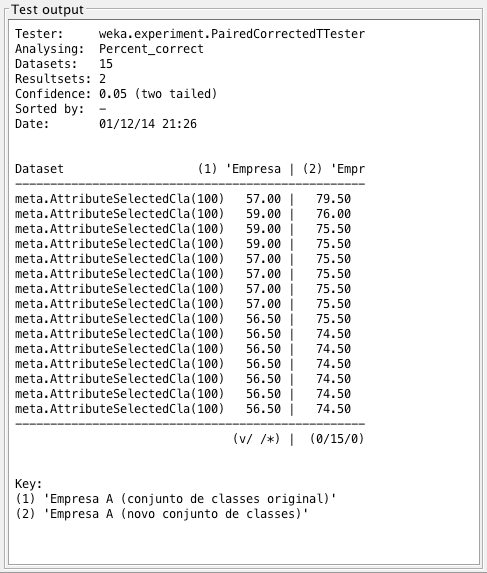
\includegraphics[width=\textwidth]{figs/geral/exaustive-j48.png}
	\caption{\label{fig_5}Aplicação exaustiva do J48}
\end{figure}

\begin{figure}[p]
	\centering
	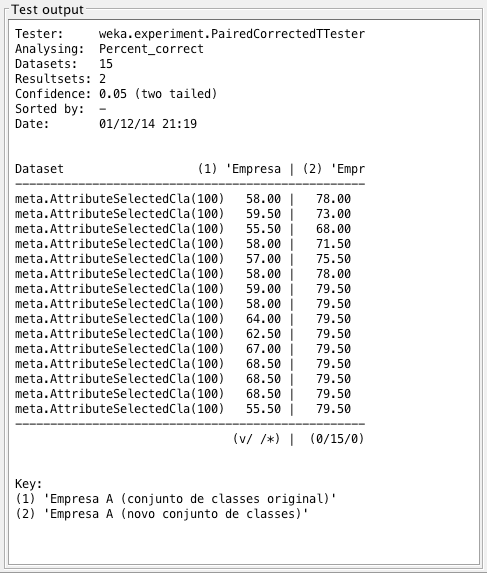
\includegraphics[width=\textwidth]{figs/geral/exaustive-naivebayes.png}
	\caption{\label{fig_6}Aplicação exaustiva do NaïveBayes}
\end{figure}
